\documentclass{beamer}

\usepackage{préambule}
\usepackage{tkz-tab}

\begin{document}

\begin{frame}
	\squared{Prendre l'énoncé}

	Résoudre les équations suivantes :
	\begin{enumerate}
		\item $(3x + 5)² = 0$
		\item $(-x - 7)² = -100$
		\item $-9x² - 3x = 0$
		\item $(x + 2)(3x - 7) = 0$
		\item $5x² - 25 = 0$
		\item $2x² + 32 = 0$
	\end{enumerate}
\end{frame}

\begin{frame}
	\squared{Prendre l'énoncé}

	Résoudre les équations suivantes :
	\begin{enumerate}
		\item $(x - 2)³ = 70$
		\item $(3x + 1)³ = -8000$
		\item $x(x+2)(x-1) = 0$
		\item $x³ + 3x² = 0$
	\end{enumerate}
\end{frame}

\begin{frame}
	\squared{Prendre l'énoncé}

	Soit $f$ la fonction définie par $f(x) = x² + 6x + 2$.
	\begin{enumerate}
		\item Déterminer les coordonnées du point le plus bas de la courbe de $f$.
		\item En déduire le tableau de variation de $f$.
		\item Résoudre l'équation $f(x) = 2$.
	\end{enumerate}
\end{frame}

\begin{frame}
	\squared{Prendre l'énoncé}

	Soit $P$ la fonction définie par $P(x) = -x³ + 6x² - 9x + k$, où $k$ est un nombre réel.
	\begin{enumerate}
		\item Déterminer la valeur de $k$ pour que $x = 4$ soit une racine de $P$. \correction{$k = 4$}
		\item On admet que $P(x) = -(x - 1)(x - 1)(x - r)$. Déterminer la valeur de $r$. \correction{$r = -4$}
		\item Remplir alors le tableau de signes suivant :

		      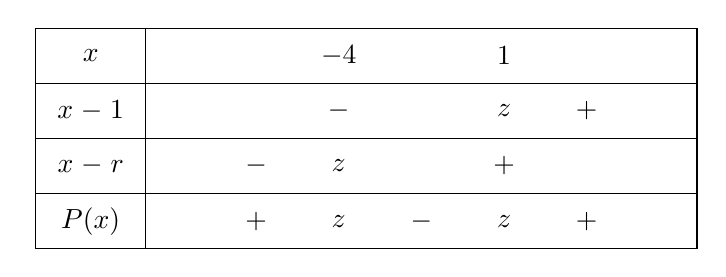
\begin{tikzpicture}[scale=0.7]
			      \tkzTabInit{$x$ / 1 , $x - 1$ / 1 , $x - r$ / 1 , $P(x)$ / 1}{, $\correction{-4}$, $\correction{1}$, }
			      \tkzTabLine{, , \correction{-}, , \correctionOr{z}{}, \correction{+}, }
			      \tkzTabLine{, \correction{-}, \correctionOr{z}{}, , \correction{+}, , }
			      \tkzTabLine{, \correction{+}, \correctionOr{z}{}, \correction{-}, \correctionOr{z}{}, \correction{+}, }
		      \end{tikzpicture}
	\end{enumerate}
\end{frame}

\end{document}